\section{Preliminaries and Related Work}\label{back}
% 
A discrete convolution is a function of two arguments: an input $u$ signal of length $L$ and a learnable filter $h$. The linear (aperiodic) convolution of a (possibly infinitely long) measurable\footnote{In the $L^1(\bZ)$ sense: $\sum_{t=-\infty}^\infty |h_t|<\infty$} filter $h$ with a length-$L$ input signal $u$ is defined as
%
\begin{equation}\label{eq:cnn}
    \begin{aligned} 
        y_t = (h * u)_t = \sum_{n=0}^{L-1} h_{t -n} u_n.
    \end{aligned}
\end{equation}
%

Generally, $u_t\in\R^D$ where $D$ is the width of the signal, or in deep learning parlance, the number of \textit{channels}. Without loss of generality, we specialize our analysis to \textit{single input single output} (SISO) layers, i.e. with $D=1$. The \textit{multiple input multiple output} (MIMO) case, canonical in standard convolutional layers, follows directly.
%

In this case, the input signal can be represented as a vector $u\in\R^L$ and the convolution as a matrix-vector product between the input and the Toeplitz kernel matrix $\sS_h \in \R^{L \times L}$ induced by the filter $h$:
%
\begin{equation}\label{eq:cnn_matvec}
    \begin{aligned} 
        %
        (h * u) = 
        %
        \begin{bmatrix}
            h_0 & h_{-1} & \cdots & h_{-L+1} \\
            h_1 & h_0 & \cdots & h_{-L+2} \\
            \vdots & \vdots & \ddots & \vdots \\
            h_{L-1} & h_{L-2} & \cdots & h_{0}
        \end{bmatrix}
        \begin{bmatrix}
            u_0\\
            u_1\\
            \vdots\\
            u_{L-1}
        \end{bmatrix}
    \end{aligned}
\end{equation}
%
\subsection{Explicit and Implicit Convolutions}
%
Parametrizing and optimizing convolution filters $h_t$ is a standard procedure in deep learning and more broadly signal processing. The classical approach of \textit{convolutional neural networks} (CNNs)  \citep{fukushima1982neocognitron,lecun1998gradient,ronneberger2015u,he2016deep} is to optimize directly the values $h_t$ of the filter's response at $M$ prescribed steps, a parametrization we call \textit{explicit}. $M$ is referred to as the \textit{filter size} and is typically much shorter than the input sequence length $M \ll L$. Such filters are denoted in signal processing as \textit{finite impulse response} (FIR). 

FIR filters are local and can capture dependencies between inputs separated at most by $M$ steps.
Their main advantage is their speed, with complexity $\mathcal{O}(ML)$. However, the number of parameters of FIR filters scales linearly with filter size, which can be computationally prohibitive. To disentangle the parameter count from the filter size, we can instead represent the filter $h_t$ as a parametric function of the time step $t$, i.e. $h_t = \gamma_\theta(t)$, where $\theta$ are the parameters of the function $\gamma_\theta$. This parametrization is called \textit{implicit}. The class of functions $\gamma_\theta$ is a design choice with a significant impact on the expressivity and computational complexity of the layer. 

One choice of implicit parametrization is to select $h$ as the response function of a linear state-space model (SSM) \citep{chen1984linear}, described by the first-order difference equation:
%
\begin{equation*}%\label{eq:ssm}
    %
    \begin{aligned}
        x_{t+1} &= \sA x_t + \sB u_t &&~~ \text{state equation} & \\
        y_t &= \sC x_t + \sD u_t &&~~ \text{output equation} &
    \end{aligned}
    %
\end{equation*}
%
Here, the convenient choice of $x_0 = 0$ renders the input-output map to a simple convolution
%
\[
    \begin{aligned}
        y_t & =\sum_{n=0}^{t}\left(\sC\sA^{t - n}\sB + \sD \delta_{t-n}\right)u_n 
    \end{aligned}
\]
%
where $\delta_t$ denotes the Kronecker delta. We can then identify the filter $h$ as
%
\[
    t\mapsto h_t =
    \begin{cases}
        0 & t<0\\
        \sC \sA^t \sB + \sD\delta_t & t\geq 0
    \end{cases}
\]
%
where the entries of $\sA, \sB, \sC$ and $\sD$ are the learned parameters of the filter. In terms of layer design, the degrees of freedom of SSMs are the dimension of the state and the structure of the matrices. 
SSMs are a canonical example of how long convolutions with sub-linear parameter counts can improve deep learning models for long sequences \citep{gu2020hippo,gu2021efficiently}.
%
 Other implicit approaches include parametrizing filters as maps from (a positional encoding of) $t$ to the filter response i.e.  $\gamma_\theta : t \mapsto h_t=\gamma_\theta(t)$, for example with feed-forward neural networks \citep{romero2021ckconv,romero2021flexconv}. 
%
\begin{tcolorbox}[enhanced, drop fuzzy shadow, frame hidden, sharp corners, breakable, colback=blue!5] \textbf{Long convolutions and memory:} A crude proxy for \textit{memory} of a single computational unit is how far in the past it can access information to produce the output at a certain step. This can be roughly quantified by the number of non-zero entries $\partial y_t / \partial u_{t-n}$ for $n = 0, \ldots, t$. The memory of CNNs filters is equivalent to the filter size $M$ since $\partial y_t / \partial u_{t-n} = h_{n}$. The total mnemonic capacity of an all-convolutions CNN therefore scales with the number of model's parameters. Implicit parametrizations, on the other hand, allow us to disentangle the memory of each filter from the parameter count and where the length of the filter is implicitly controlled by the learned parameters. In an SSM, $\partial y_t / \partial u_{t-n} = \sC \sA^n \sB$ and the memory extent is solely determined by the spectral radius of $\sA$ and can be finely tuned by the training process\footnote{See e.g.\cite{gu2020hippo,gu2021efficiently}}. On the other hand, the number of parameters controls the \textit{expressivity} of the memory unit, e.g. the number of basis functions forming $h_t$. 
\end{tcolorbox}
%
\paragraph{Fast Methods for Convolutions}
%
One of the first applications of the Cooley-Tukey fast Fourier transform (FFT) algorithm was to implement convolution faster than the direct evaluation of \eqref{eq:cnn}.
At first glance \eqref{eq:cnn} comes with $O(L^2)$ an asymptotic time complexity. 
A common approach to achieve \textit{fast long convolutions} in subquadratic time is through the FFT algorithm. The method first converts the \textit{aperiodic} convolution into a \textit{circular} convolution \cite{selesnick2017fast} by appropriate zero-padding of input and filter sequences. The resulting kernel $\hat\sS_h$ is a circulant matrix and is diagonalized by the discrete Fourier basis
%
\[
    \hat \sS_h = \sW^{-1} \sD_{H} \sW
\]
%
where $\sW$ is the DFT matrix, $\sW_{tt'} = z^{-t}, z = e^{i2\pi t'/L}$ and $H$ is the DFT of the padded filter $h$, $H = \sW {\sf pad}(h)$. Thus, the calculation of such convolutions is performed as
%
\begin{equation*}
    \begin{aligned}
        {\sf pad}(y) &= \hat \sS_h {\sf pad}(u) \\
        &= \sW^{-1}\sD_H \sW ~{\sf pad}(u)\\
        &= {\sf iFFT}(\sD_H {\sf FFT}({\sf pad}(u)))
    \end{aligned}
\end{equation*}
%
where $\sD_H$ is the matrix with $\sW h$ on its diagonal. The above is known as the convolution theorem of DFT \citep{oppenheim1997signals}. In this ${\sf FFTConv}$ form the convolution can be performed \textbf{without materializing the operator $\sS_h$} with the same asymptotic cost $O(L\log_2 L)$ of FFT.
%
\subsection{The Self-Attention Operator}
%
At the heart of Transformers is the \textit{multi-head attention} (MHA) mechanism. Given a length-$L$ sequence $u\in\R^{L\times D}$, each \textit{head} of \textit{scaled self-attention} \citep{vaswani2017attention} is a map from $\R^{L\times D}$ to $\R^{L\times D}$ which performs the following operations
%
\begin{equation}\label{eq:att}
    \begin{aligned}
      %&{\sf SelfAttention}: \R^{L\x D}\rightarrow \R^{L\x D} \\
      \sA(u) &= {\sf SoftMax}\left(\tfrac{1}{\sqrt{D}}u \sM_q \sM^\top_k u^\top \right)\\
      y &= {\sf SelfAttention}(u) \\
        &= \sA(u)u \sM_v,
    \end{aligned}
\end{equation}
%
\begin{figure*}[t]
    \centering
    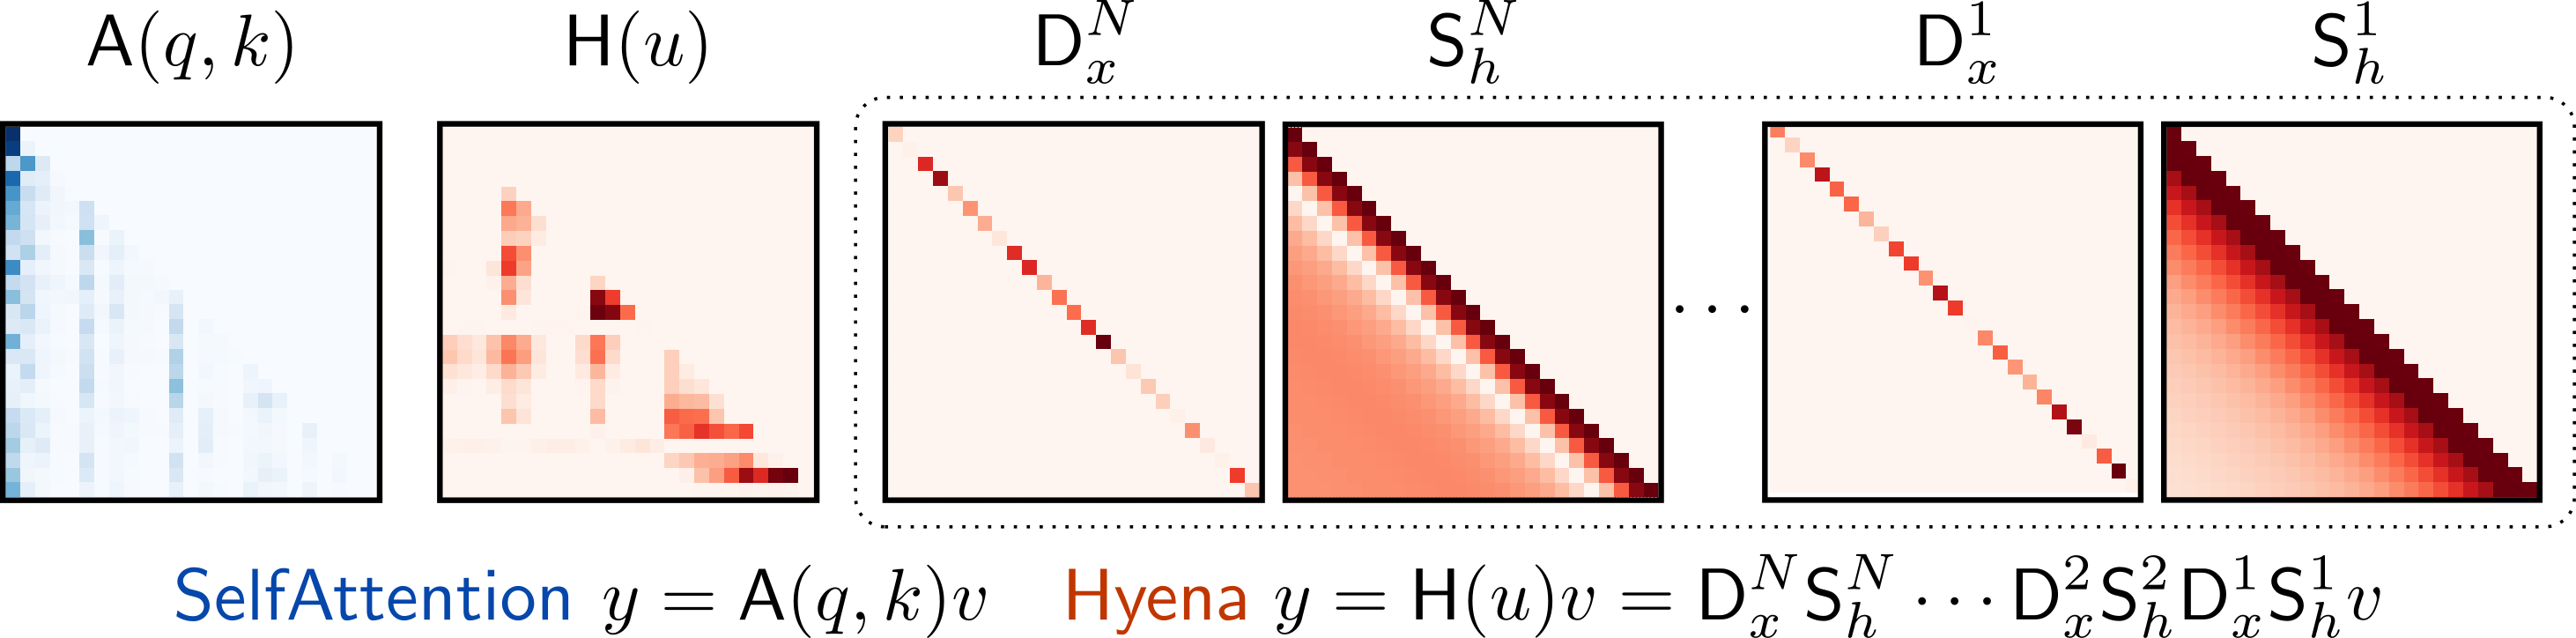
\includegraphics[width=0.69\linewidth]{figures/attention.png}
    \vspace{-2mm}
    \caption{Comparison between data-controlled matrices: $\sf SelfAttention$ and $\sf Hyena$.}
    \label{fig:hyena_matrices}
\end{figure*}
%
where $\sM_q, \sM_k, \sM_v\in\R^{D\x D}$ are learnable linear projections and ${\sf SoftMax}$ is intended to be applied row-wise. Attention parametrizes a \textbf{family of dense linear operators} and for an input $u$, indexes through it via projections of $u$ i.e., $\sA(u)$. We refer to operators of this type as \textit{data-controlled}, as they encode a linear transformation $u \mapsto y$, that is, however, nonlinearly defined by $u$. This approach yields expressive nonlinear operators in $u$, and we hypothesize contributes, together with other mechanisms \citep{olsson2022context}, to the ability of certain operators to learn \textit{in-context} i.e., to adapt to unseen tasks by leveraging context. In deep learning, the projections take on specific names: \textit{query} $q=u\sM_q$, \textit{key} $k=u\sM_k$ and \textit{value} $v = u\sM_v$. We often rewrite the attention operator as $y = \sA(q,k)v$.
%
\begin{remark}
    Similarly to implicit convolutions, $\sf SelfAttention$ does not entangle its ability to access distant information with the number of parameters: it looks at the whole sequence at the price of $\cO(L^2)$ operations.
\end{remark}
%
\paragraph{Subquadratic Operators}
%
Existing approaches to subquadratic alternatives to attention can be summarized by altering the way the data control is implemented i.e., how the operator is nonlinearly defined by $u$, and then applied to $v$. For example, a layer of \textit{Attention-Free Transformers} (AFTs) \citep{zhai2021attention} constructs the operator through a combination of gating and {$\sf SoftMax$} (AFT full) or gating and a single explicit convolution (AFT conv). \textit{Gated State Spaces} (GSS) instead compose the operator via gating and a long convolution parametrized via SSMs. Taking this idea further, \textit{Hungry Hungry Hippo (H3)} \citep{dao2022hungry}, motivated by gaps of GSS on associative recall, extend the mechanism to include an additional gate and a short convolution obtained via a shift SSM. ${\sf Hyena}$ generalizes this body of work by introducing a recurrence of gates and implicit long convolutions, evaluated efficiently.